\chapter{Virtualizzazione}
\section{Cosa è?}
La virtualizzazione è una tecnologia che crea istanze logiche e astratte delle risorse fisiche di caclolo.

Si avvale di un \textbf{hypervisor} (o Virtual Machine Monitor) per \underline{partizionare l'hardware fisico e creare più ambienti virtuali isolati}, le machine virtuali.

Ogni VM esegue il proprio sistema operativo e le proprie applicazioni nella convinzione di disporre di hardware dedicato, pur condividendo le risorse fisiche sottostanti.

\section{Perchè virtualizzare?}
La virtualizzazione è anzitutto uno strumento di economia delle risorse e di disaccoppiamento fra software e hardware sottostante

\begin{itemize}
    \item \textbf{Consolidamento (Più carichi su un nodo)} \\
    I server x86 dedicati sono utilizzati in media al 5--15\,\%. Il consolidamento alza l'utilizzo a 60--80\,\%, con riduzione di \textit{capex}, energia, raffreddamento e spazio fisico.
    
    \item \textbf{Isolamento (Confinamento dei guasti)} \\
    Crash, panic e exploit di un guest non si propagano agli altri. Il VMM fornisce un \textit{fault domain} più stretto del processo Unix tradizionale.
    
    \item \textbf{Multi-tenancy (Isolamento)} \\
    Tenant mutuamente non fidati condividono lo stesso hardware fisico.
    
    \item \textbf{Mobilità (Disaccoppiamento HW/SW)} \\
    Snapshot, clonazione, migrazione \textit{live}: una VM è un file portabile. Manutenzione hardware senza downtime applicativo.
    
    \item \textbf{Compatibilità (Sistemi legacy)} \\
    Esecuzione di OS obsoleti su hardware moderno; ambienti di sviluppo riproducibili; emulazione di ISA estranee (es. ARM su x86).
\end{itemize}

\subsection{Consolidamento e multi-tenacy}
\begin{minipage}[c]{0.5\textwidth}
    \begin{itemize}
        \item La virtualizzazione permette di consolidare più macchine virtuali su un singolo sistema  fisico, riducendo il total cost of ownership (TCO)
        \item TCO: stima di tutti i costi diretti e indiretti legati all'acquisto e all'esercizio di un prodotto o sistema lungo l'intero ciclo di vita
    \end{itemize}
\end{minipage}
\hfill
\begin{minipage}[c]{0.5\textwidth}
        \centering
        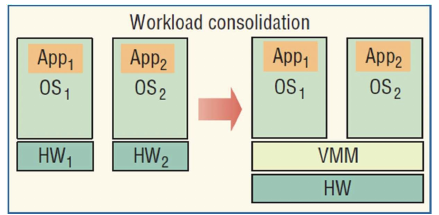
\includegraphics[scale=0.75]{figures/Schermata_20260608_122606.png}
\end{minipage}

\subsection{Isolamento dei carichi di lavoro}
\begin{minipage}[c]{0.5\textwidth}
    \begin{itemize}
        \item Grazie alla virtualizzazione si ottiene l'isolamento del carico di lavoro: \uline{tutte le istruzioni di un programma restano confinate all'interno della VM}
        \item \textbf{Affidabilità}: i guasti software all'interno di una VM non si propagano alle altre
        \item \textbf{Controllo delle prestazioni}: l'esecuzione di una VM non deve incidere sulle prestazioni di un altra VM
    \end{itemize}
\end{minipage}
\hfill
\begin{minipage}[c]{0.5\textwidth}
    \begin{center}
        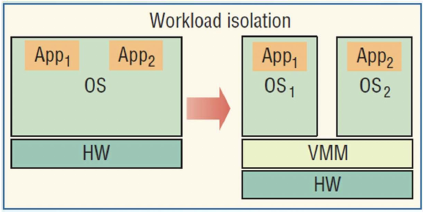
\includegraphics[scale=0.75]{figures/Schermata_20260608_123244.png}
    \end{center}
\end{minipage}


\subsection{Gestione della "sessione"}
La VM è un file il cui stato si può congelare, replicare, ripetere, 3 primitive ne reggono l'operatività nel cluster:
\begin{itemize}
    \item \textbf{Snapshot - stato istantaneo} 
    \begin{itemize}
        \item Cattura sincrona di memoria, registri, disco. \\
        Il disco usa copu-on-write \\ 
        Rollback in meno di un secondo
    \end{itemize}
    \item \textbf{Checkpoint - snapshot persistente}
    \begin{itemize}
        \item Snapshot serializzato su storage durevole, con stato di rete e device. \\
        Abilita resume dopo spegnimento, debug record-and-replay, "criogenia" delle VM
    \end{itemize}
    \item \textbf{Faul Tolerance - replica continua}
    \begin{itemize}
        \item VM secondaria mantuenuta sincronizzata. \\
        Se cade il primario, il secondario subentra senza perdita di stato osservabile
    \end{itemize}
\end{itemize}

\section{Migrazione dei carichi di lavoro}
\begin{minipage}[c]{0.4\textwidth}
    La migrazione del carico di lavoro (application mobility) migliore: 
\begin{itemize}
    \item La manutenzione hardware
    \item Le prestazioni
    \item La fault tollerance
\end{itemize}  
\end{minipage}
\hfill
\begin{minipage}[c]{0.6\textwidth}
    \centering
    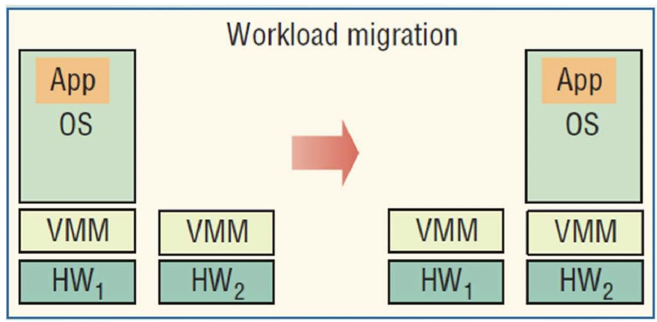
\includegraphics[scale=0.65]{figures/Schermata_20260608_124411.png}
\end{minipage}
Si realizza permettendo al guest OS di una VM di essere sospeso, migrato su un'altra piattaforma e ripreso immediatamente, oppure conservato per essere ripristinato in un secondo momento.

\section{Strategie di migrazione}
\subsection{Strategia Pre-copy}
\begin{minipage}[c]{0.5\textwidth}
    \begin{enumerate}
        \item \textbf{Push} \\
        Copia delle pagine di memoria verso la destinazione mentre la VM continua a girare
        \item \textbf{Dirty Pages}\\
        Reinvio delle pagine modificate durante la copia iniziale
        \item \textbf{Stop-and-copy} \\
        Breve interruzione (downtime per copiare le ultime pagine residue e traferire il controllo)
        \item \textbf{Risultato} \\
        Tempi di inattività minimi
    \end{enumerate}

\subsubsection{Migrazione delle risorse locali}
    \begin{itemize}
        \item \textbf{Netowrking:}\\
        Annuncio del nuovo binding indirizzo-MAC o tunneling/mobile IP per mantenere attive le connessioni
        \item \textbf{Storage:}\\
        Tipicamente risolto separando lo storage in un livello dedicato. \\
        La migrazione richiede solo di ristabilire la connessione di rete verso il server di storage, senza trasferire fisicamente i file
    \end{itemize}
\end{minipage}
\hfill
\begin{minipage}[c]{0.5\textwidth}
    \centering
    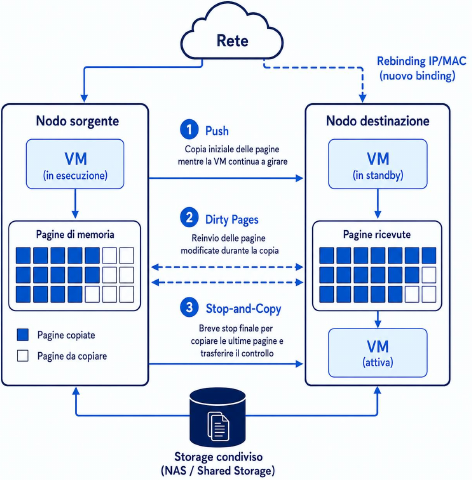
\includegraphics[scale=0.8]{figures/Schermata_20260608_153424.png}
\end{minipage}

\newpage
\subsection{Strategia Post-copy}
\begin{minipage}[c]{0.5\textwidth}
    \begin{enumerate}
        \item \textbf{Stop \& Switch:}\\
        La VM viene sospesa e si trasferisce subito solo lo stato minimo (CPU, registri, device)
        \item \textbf{Demand Paging:}\\
        La VM riparte sulla destinazione, le pagine mancanti vengono richieste all'origine via rete
        \item \textbf{Background Push:}\\
        In parallelo l'origine spinge proattivamente le pagine restanti per ridurre i fault
        \item \textbf{Risultato:}
        Downtime molto breve, ma performance degradate fichè il trasferimento non è completo
    \end{enumerate}

    \subsubsection{Migrazione delle risorse locali}
    \begin{itemize}
        \item \textbf{Networking:}\\
        Annuncio del nuovo binding indirizzo-MAC o tunneling/mobile IP per mantenere attive le connessioni
        \item \textbf{Storage:}\\
        Tipicamente risolto separando lo storage in un livello dedicato.\\
        La migrazione richiede solo di ristabilire la connessione di rete verso il server di storage, senza trasferire fisicamente i file
    \end{itemize}
\end{minipage}
\hfill
\begin{minipage}[c]{0.5\textwidth}
    \centering
    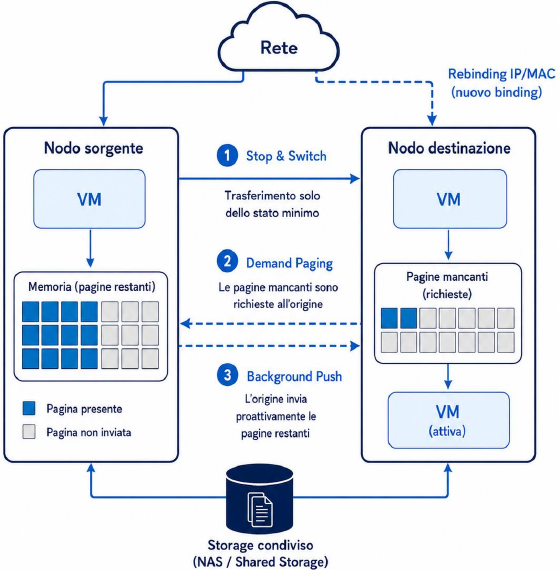
\includegraphics[scale=0.7]{figures/Schermata_20260608_154419.png}
\end{minipage}

\subsection{Consolidamento dinamico}
La live migration permette di riorganizzare le VM tra gli host mentre tutto è in esecuzione: si possono accendere e spegnere server a secondo del carico senza fermare i servizi.

\begin{itemize}
    \item \textbf{Obiettivo:}\\
    Concentrare le VM attive sul minor numero possibile di host, così quelli vuoti possono essere spenti per risparmiare energia
    \item \textbf{Meccanismo:}\\
    Lo scheduler del cluster controlla periodicamente il carico e, se è opportuno, sposta a caldo alcune VM verso altri host
    \item \textbf{Quando scatta:}\\
    Quando un host è sotto/sovra-utilizzato
\end{itemize}

\section{Cos'è un hypervisor?}
Un hypervisor (o Virtual Machine Monitor) è un componente \underline{software che crea e gestisce le macchine virtuali} astraendo e partizionando le risorse hardware fisiche.

Sfrutta le estensioni hardware per la virtualizzazione offerte dalle CPU moderne per gestire le VM in modo efficiente, fa questo condividendo le risorse disponibili in modo che ciascuna VM le percepisca come dedicate

\section{Tassonomia degli hypervisor}
La tassonomia di Goldberg distingue gli hypervisor in base alla loro relazione con l'hardware

\subsection{Architettura bare-metal}
\begin{minipage}[c]{0.5\textwidth}
    In questa architettura l'hypervisor è \uline{installato direttamente sull'hardware nudo e dialoga direttamente con l'hardware} del sistema senza appoggiarsi a un host OS diventando \textbf{praticamente un OS leggeto}.
\end{minipage}
\hfill
\begin{minipage}[c]{0.5\textwidth}
    \begin{figure}[H]
        \centering
        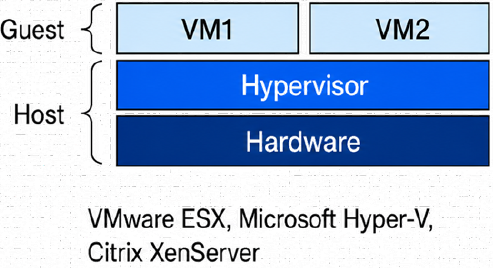
\includegraphics[scale=0.5]{figures/Schermata_20260608_115837.png}
    \end{figure}
\end{minipage}


\begin{itemize}
    \item \textbf{Vantaggi}
    \begin{itemize}
        \item Migliore prestazioni di I/O
    \end{itemize}
    \item \textbf{Svantaggi}
    \begin{itemize}
        \item Installazione e configurazione complesse
        \item Forte dipendenza dalla piattaforma hardware
    \end{itemize}
\end{itemize}

\subsection{Architettura hosted}
\begin{minipage}[c]{0.5\textwidth}
    Si installa per il primo sistema operativo host, l'hypervisor viene installato sopra il sistema operativo host.

    Permette agli utenti di \uline{eseguire diversi sistemi operativi guest in parallello}
\end{minipage}
\hfill
\begin{minipage}[c]{0.5\textwidth}
    \begin{figure}[H]
        \centering
        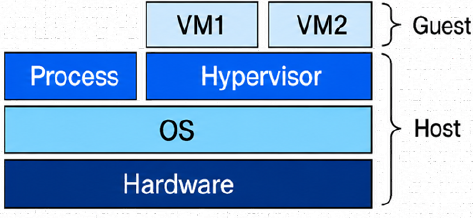
\includegraphics[scale=0.5]{figures/Schermata_20260608_120709.png}
    \end{figure}
\end{minipage}

\begin{itemize}
    \item \textbf{Vantaggi}
    \begin{itemize}
        \item Installazione e configurazioni semplici
        \item Host OS e guest OS non modificati
        \item Esecuzione su un'ampia gamma di computer
    \end{itemize}
    \item \textbf{Svantaggi}
    \begin{itemize}
        \item Decadimento delle prestazioni
    \end{itemize}
\end{itemize}

\section{Cosa fa una macchina virtuale?}
Una macchina virtuale fornisce una piattaforma hardware emulata completa, in grado di ospitare un sistema operativo a tutti gli effetti.
\begin{itemize}
    \item Le risorse della macchina fisica sottostante possono essere condivise tra più macchine virtuali, ciascuna con un proprio sistema operativo
    \item Create e gestite da un hypervisor
\end{itemize}

\subsection{Proprietà}
\begin{itemize}
    \item \textbf{Equivalenza}

    Un programma in esecuzione nella VM mostra un comportamente essenzialmente identico a quello osservabile sulla macchina fisica, eccezion fatta per gli effetti di temporizzazione e di disponibilità delle risorse

    \item \textbf{Controllo delle risorse}

    Il VMM mantiene il controllo completo delle risorse fisiche: nessun programma guest può accedere a risorse non esplicitamente allocate, né alterare l'allocazione decisa dal VMM

    \item \textbf{Efficienza}
    
    Una frazione statisticamente dominante delle istruzioni macchina è eseguita direttamente dal processore fisico, senza intervento del VMM
\end{itemize}

\section{Process Virtual Machine}
Una process virtual machine (o application VM) fornisce un ambiente di esecuzione indipendente dalla piattaforma per una singola applicazione.

A differenza della system VM, che virtualizza l'intero hardware, \uline{virtualizzano solo ciò che serve a quella applicazione}.

\subsection{Proprietà}
\begin{itemize}
    \item \textbf{Singola applicazione}: ogni istanza esegue un solo processo
    \item \textbf{Indipendenza dalla piattaforma}: \texttt{<<write once, run everywhere>>}, ovunque sia disponibile la VM
    \item \textbf{Esecuzione gestita}: memoria, garbage collection e sicurezza forniti dal runtime
    \item \textbf{Rappresentazione intermedia}: il codice è compilato in bytecode, interpretato o compilato just-in-time dalla VM
\end{itemize}

\section{Classificazione delle istruzioni}
Le istruzioni si classificano in base al \uline{privilegio richiesto e la sensibilità verso lo stato della macchina}

\begin{figure}[H]
    \centering
    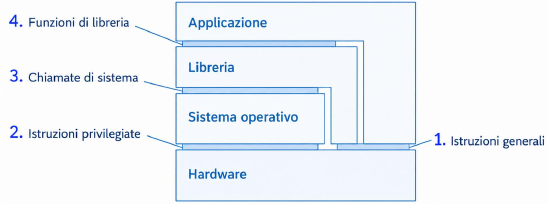
\includegraphics[width=1\textwidth]{figures/Schermata_20260608_110233.png}
\end{figure}

\begin{itemize}
    \item \textbf{Asse privilegio}
    \begin{itemize}
        \item Le \uline{privilegiate} generano una trap se eseguite in user mode
        \item Le \uline{non privilegiate} vengono eseguite direttamente dalla CPU
    \end{itemize}
    \item \textbf{Asse sensibilità}
    \begin{itemize}
        \item Le \uline{sensibili} influiscono sull'hardware condiviso fra le VM: accedendo o modificando registri di sistema, memoria della macchina, interrupt
        \item Le \uline{innocue} restano dentro la VM: calcoli, salti. lettura e scrittura sulla propria memoria
    \end{itemize}
\end{itemize}

\section{CPU protection ring}
Le CPU moderne definiscono livelli di protezione (ring) che vanno da 0 (massimo privilegio) a 3 (privilegio minimo).

Il kernel dei sistemi operativi sono progettati per girare in Ring 0 ed eseguire le istruzioni privilegiate direttamente sull'hardware

\subsection{Applicazione alle VM}
In un ambiente virtualizzato il guest OS crede di avere il pieno controllo dell'hardware, ma in realtà gira in \textbf{modalità deprivilegiata}.


L'hypervisor deve intercettare queste istruzioni ed eseguire un \textbf{trap-and-emulate}, per le istruzioni sensibili invece:
\begin{itemize}
    \item \textbf{Traduzione binaria}
    \item \textbf{Paravirtualizzazione}
    \item \textbf{Virtualizzazione assistita dall'hardware}
\end{itemize}

\subsection{Modalità di esecuzione}
\begin{itemize}
    \item \textbf{Root mode}

    Esegue l'hypervisor, con pieno accesso all'hardware reale

    \item \textbf{Non-root mode}

    Esegue il guest, che usa normalmente i ring x86.

    Le operazioni richiedo l'intervento dell'hypervisor sono però intercettate dalla CPU
\end{itemize}

\subsection{VM-exit}
Transizione hardware da non-root a root: la CPU sospende il guest e cede il controllo all'hypervisor.

Può essere causata da istruzioni privilegiate, accessi I/O, eventi sulla memoria, interrupt, timer, o politiche configurate dall'hypervisor.

Il trapping avviene in hardware, la gestione dell'evento resta software


Quando il guestOS tenta di eseguire un'istruzione privilegiata, la \uline{CPU genera un trap} (eccezione) che trasferisce il controllo all'hypervisor, il quale \textbf{emula} il comportamento dell'istruzione in modo sicuro e virtualizzato.

\section{Trap-and-emulate}
\subsection{Obiettivo}
Permettere a un sistema operativo guest di eseguire codice come se avesse il controllo dell'hardware fisico

\begin{figure}[H]
    \centering
    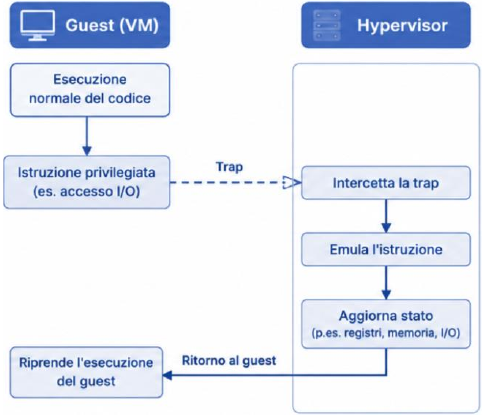
\includegraphics[scale=0.6]{figures/Schermata_20260608_111337.png}
\end{figure}

\subsection{Esecuzione normale}
Le istruzioni non privilegiate del guest vengono eseguite direttamente dalla CPU, senza intervento continuo dell'hypervisor

\subsection{Trap}
Quando il guest esegue un'istruzione privilegiata o accede a una risorsa protetta, la CPU genera un trap e trasferisce il controllo all'hypervisor

\subsection{Emulate}
L'hypervisor interpreta la richiesta, aggiorna lo stato virtuale della VM ed emula l'effetto dell'operazione sull'hardware virtuale

\section{Traduzione binaria dinamica}
\subsection{Cosa è?}
La traduzione binaria è una tecnica di virtualizzazione che, a tempo di esecuzione scansiona, analizza e riscrive dinamicamente il codice del guest, sostituendo le istruzioni problematiche con equivalenti sicuri eseguibili in un ambiente virtualizzato.

\subsection{Obiettivo}
Eseguire un sistema guest quando alcune istruzioni sensibili non sono virtualizzabili con il solo trap-and-emulate

\begin{figure}[H]
    \centering
    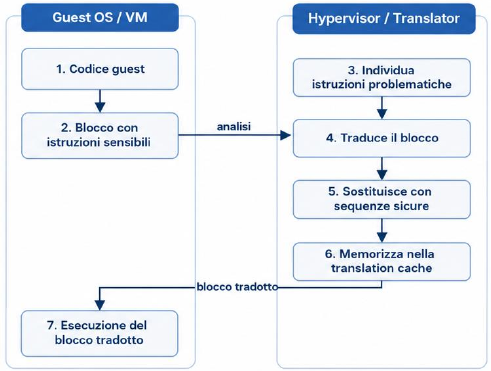
\includegraphics[scale=.75]{figures/Schermata_20260608_112010.png}
\end{figure}

\subsection{Idea base}
L'hypervisor analizza il codice e riscrive i blocchi con istruzioni problematiche, sostituendoli con sequenze sicure.

\subsection{Flusso}
Il guest esegue codice normale, sui blocchi sensibili il traduttore produce una versione equivalente sicura, che viene eseguita al loro posto

\subsection{Vantaggio}
Virtualizza architettura come lo x86 classico, dove alcune istruzioni sensibili non generano trap in modo affibile

\subsection{Costo}
Più complesso del trap-and-emulate: 
\begin{itemize}
    \item overhead per traduzione
    \item cache dei blocchi
    \item gestione del controllo
\end{itemize}

\section{Paravirtualizzazione}
\subsection{Idea}
La paravirtualizzazione è una tecinca di virtualizzazione in cui il sistema operativo guest viene modificato per essere consapevole di girare un ambiente virtualizzato.

\subsection{Hypercall}
Il guest usa \uline{chiamate speciali per interagire direttamente con l'hypervisor}, queste chiamate prendono il nome di \textbf{hypercall}

\subsection{Come procede il guest?}
I sistemi operativi guest sono consapevoli dell'hypervisor e utilizzano chiamate speciali per interagire con esso, questo si traduce in:
\begin{itemize}
    \item migliori prestazioni
    \item integrazione fluida
    \item sicurezza ridotta
\end{itemize}

